

\section{Percepção dos desenvolvedores em relação as vulnerabilidade em aplicativos open source}

O artigo "Perceptions of Software Practitioners Regarding Crypto-API Misuses and Vulnerabilities" aborda a percepção dos desenvolvedores e profissionais de segurança em relação às vulnerabilidades em aplicativos open source. O estudo não se limitou apenas à análise estática das ferramentas utilizadas, mas também incluiu uma investigação sobre aplicativos Android de código aberto, com o objetivo de obter a opinião dos desenvolvedores envolvidos.

Uma descoberta relevante foi que muitas das questões identificadas pelo CogniCrypt não estavam diretamente relacionadas ao código do aplicativo Android em si, mas sim às bibliotecas de terceiros utilizadas por esses aplicativos. Dentre os projetos de código aberto analisados, aproximadamente 60\% apresentaram questões levantadas pelo CogniCrypt que se originavam de códigos de terceiros. Os desenvolvedores abordaram essas preocupações de segurança de maneiras diversas. Alguns optaram por atualizar imediatamente as dependências, enquanto outros confiaram implicitamente nas grandes empresas de tecnologia fornecedoras das bibliotecas e não consideraram os problemas como ameaças reais.

Surpreendentemente, em alguns casos, os desenvolvedores tiveram dificuldades em compreender completamente as questões apresentadas pelo CogniCrypt. Para eles, não estava claro por que determinados trechos de código eram considerados problemas apenas a partir das explicações fornecidas pela ferramenta. Diante disso, os desenvolvedores expressaram o desejo de receber explicações mais detalhadas sobre os problemas identificados, bem como sugestões diretas sobre como corrigi-los. Além disso, alguns sugeriram a categorização dos problemas levantados pelo CogniCrypt com base na origem, indicando se pertencem ao aplicativo digitalizado ou a uma biblioteca de terceiros. Essa observação proporciona insights valiosos sobre a necessidade de uma comunicação mais eficaz entre as ferramentas de análise e os desenvolvedores, visando uma compreensão mais precisa e eficiente das vulnerabilidades detectadas.

\section{Análise quantitativa em aplicativos android}

Foram analisados 307 aplicativos de 6 diferentes categorias do repositório de aplicativos de código aberto F-Droid.
A execução do CogniCrypt reportou 195 Warnings de uso indevido de criptografia enquanto o CryptoGuard reportou 298.
A tabela abaixo mostra a quantidade de aplicativos analisados por categoria e a quantidade de Warnings reportados por cada ferramenta.

\begin{table}[!htbp]
  \centering
  \begin{tabular}{|c|c|c|c|}
  
    \textbf{Categoria}   & \textbf{Número de Aplicativos}   &  \textbf{CogniCrypt}     &  \textbf{CryptoGuard} \\ 
     Connectivity           & \num{58}                         &  \num{20}                    & \num{3}                     \\
Finances                & \num{90}                         &  \num{25}                    & \num{2}                     \\
Internet                 & \num{39}                         &  \num{7}                      &     \num{0}                  \\
Security                 & \num{47}                         &  \num{16}                    &     \num{1}                  \\
Sms-Phone            & \num{18}                         &  \num{10}                     &     \num{2}                 \\
System                  & \num{55}                        &   \num{34}                    &     \num{0}                  \\
\textbf{Total}        & \num{307}                      &   \num{112}                  &     \num{8}                   \\
\end{tabular}
    
  \caption{Aplicativos por categoria sem warning das ferramentas CogniCrypt e CryptoGuard}
\label{AplicativosSemWarning}
\end{table}

Como visto, o número de aplicativos sem warning no cognicrypt é bem maior do que no cryptoguard. A categoria sistema é a que tem a maior diferença entre eles, \num{34}. As categorias conectividade e finanças também tem um número alto de aplicativos sem warnings, \num{20} e \num{25}, respectivamente.

Apesar disso, o número de warnings fundados pelo CogniCrypt é maior do que no CryptoGuard, descrito na tabela abaixo.

\begin{table}[!htbp]
  \centering
  \begin{tabular}{|c|c|c|c|}
  
    \textbf{Categoria}   & \textbf{CogniCrypt (a)}   &  \textbf{CryptoGuard (b)}     &  \textbf{Diferença (a - b)} \\ 
     Connectivity           & \num{1768} (\num{16.02}\%)  &  \num{1124} (\num{22.64}\%)  & \num{644} (\num{10.61}\%) \\
Finances                &     \num{3087} (\num{27.97}\%)     &     \num{1687} (\num{33.98}\%)     &     \num{1400} (\num{23.06}\%)\\
Internet                 &     \num{3407} (\num{30.87}\%)     &     \num{916} (\num{18.45}\%)     &     \num{2491} (\num{41.02}\%)\\
Security                 &     \num{1780} (\num{16.13}\%)     &     \num{553} (\num{11.14}\%)     &     \num{1227} (\num{20.21}\%)\\
Sms-Phone            &     \num{428} (\num{3.88}\%)     &     \num{171} (\num{3.44}\%)     &     \num{257} (\num{4.23}\%)\\
System                  &     \num{566} (\num{5.13}\%)     &     \num{513} (\num{10.33}\%)     &     \num{53} (\num{0.87}\%)\\
\textbf{Total}                     &     \num{11036} (\num{100.00}\%)     &     \num{4964} (100.00\%)     &     \num{6072} (\num{100.00}\%)\\
\end{tabular}
    
  \caption{Warnings encontrados nas ferramentas CogniCrypt e CryptoGuard}
\label{AplicativosComWarning}
\end{table}

Como podemos observar na tabela acima, o CogniCrypt consegue encontrar 4964 warnings enquanto o Cryptoguard encontrou 11036 warnings. A diferença numérica é de 6072 (ou 122.32\%) de warnings entre as duas ferramentas. A categoria de finanças e internet concentrou 58.8\% (6494) dos warnings do CogniCrypt e as categorias de finanças e conectividade concentram 56.6\% (2811) dos warnings do CryptoGuard. A maior diferença entre os warnings fundados foi notada nas categorias internet (2491) e finanças (1400), representando 64.1\% de diferença. 

Considerando os resultados acima, analisamos a quantidade média de warnings por aplicativo. Os resultados são mostrados no gráfico abaixo.

\begin{figure}[!h]
    \centering
    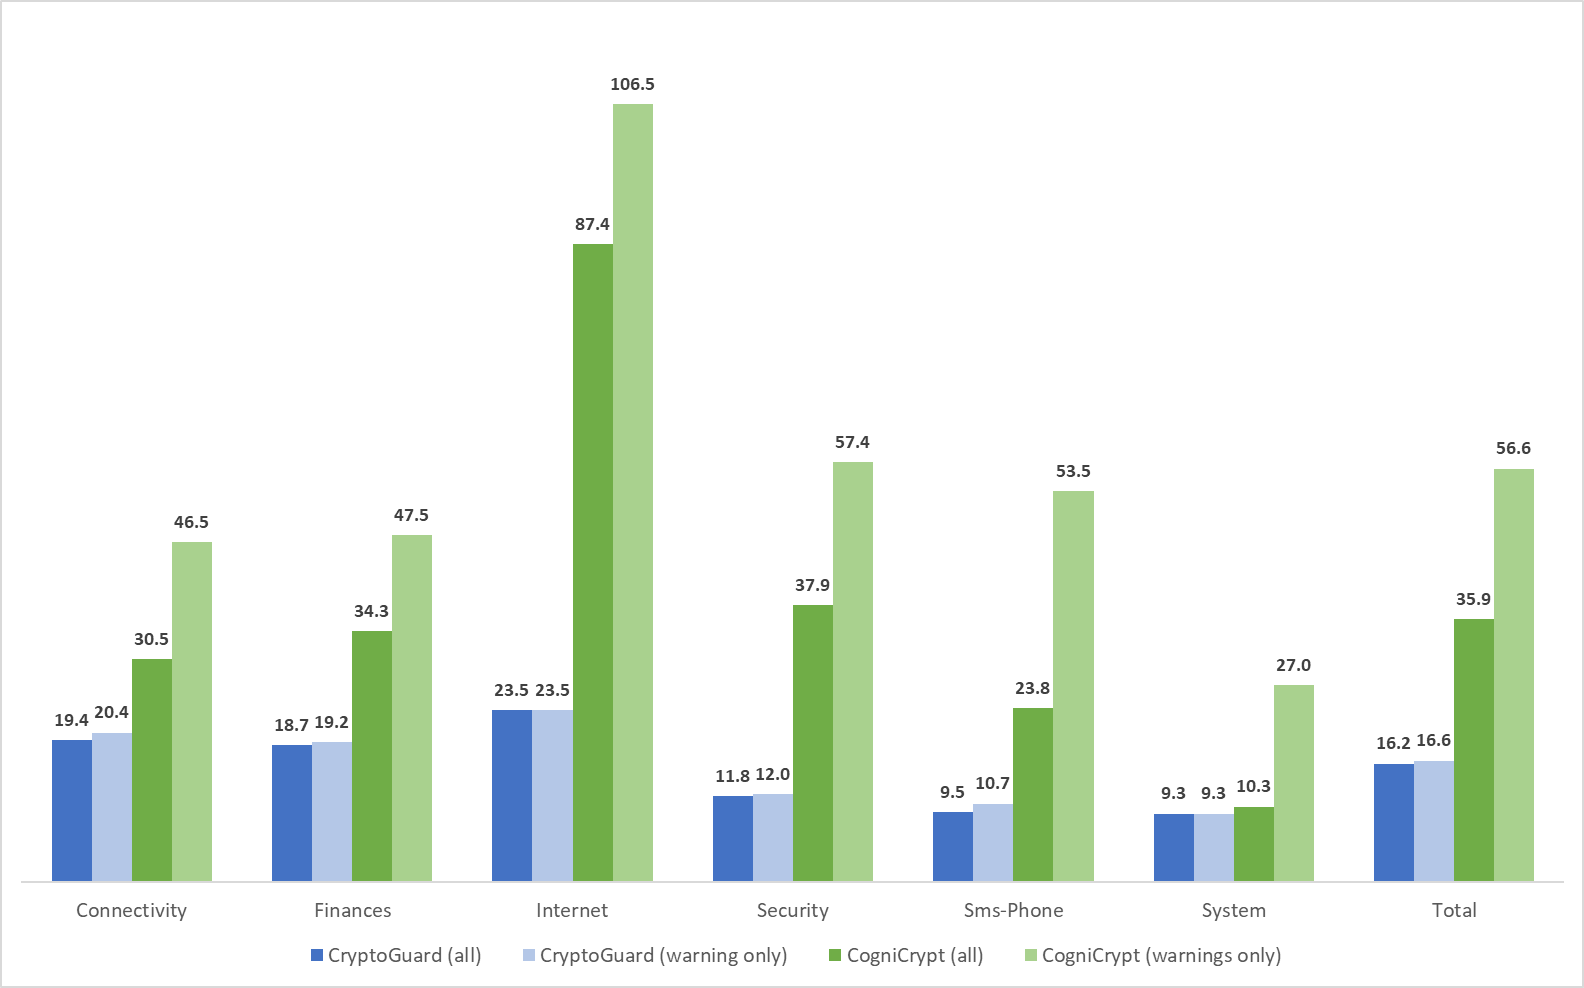
\includegraphics[scale=0.3]{images/averageWarnings.png}
    \caption{Quantidade média de alertas por aplicativo}
    \label{averageWarnings}
\end{figure}

Como esperado, a média de warnings é maior no CogniCrypt do que no CryptoGuard. A diferença é ainda maior quando desconsideramos os aplicativos sem warnings. A categoria internet tem a maior média de warnings nas duas ferramentas, com um valor maior no CogniCrypt: 106.5 warnings por aplicativo. Em segundo e terceiro lugares temos as categorias segurança e sms-telefone no CogniCrypt e internet e conectividade, considerando a média de warnings fundados pelo CryptoGuard.

\subsection{Análise da integração do Cryptoguard e do Cognicrypt com o LibScout}





% %http://aprender_unb.br/course/view.php?id=25
% %http://www.cs.berkeley.edu/~jrs/speaking.html
% Este capítulo oferece sugestões de como fazer a apresentação do trabalho. Uma
% apresentação é necessária ao final do curso, é nela que se mostra os resultados
% obtidos de forma resumida e, preferencialmente, simplificada. Embora o ``verdadeiro''
% resultado seja o texto técnico, que de fato representa a contribuição científica
% obtida, a apresentação serve para divulgar seus resultados e incentivar outros a
% se interessarem por seu trabalho.

% \section{Falando em Público}
% A ideia de uma apresentação não é mostrar todos os detalhes técnicos ou tentar
% impressionar o público com seu conhecimento. O objetivo é apresentar suas principais
% ideias de forma intuitiva, de modo que os presentes entendam o que foi feito e
% se interessem em conhecer as minúcias lendo o texto técnico.

% Vale lembrar que embora você veja seu trabalho como extremamente interessante,
% geralmente seu público [ainda] não acha, e provavelmente têm coisas melhores para fazer...
% É preciso atrair e manter a atenção deles, bem como garantir que eles se lembrem
% do que foi dito (pelo menos da ideia principal).

% Algumas noções importantes:
% \begin{description}
% \item[Motivação:] Qual o problema e por que ele merece atenção?
% \item[Ideia Principal:] Clara e explicitamente especificada.
% \item[Exemplos:] A melhor forma de passar informações (ilustram motivação,
% funcionamento, casos extremos, limitações, etc.).
% \end{description}

% \emph{Slides} são uma excelente ferramenta \textbf{de apoio} ao apresentador, mas
% muitas vezes tomam vida própria e se tornam o elemento principal. É essencial,
% embora um pouco difícil,  evitar a ``morte por Powerpoint''\footnote{%
% \url{http://www.smallbusinesscomputing.com/biztools/article.php/684871/Death-By-Powerpoint.htm}}.

% Existem muitas sugestões para fazer uma boa apresentação\footnote{\url{https://hbr.org/2014/11/how-to-give-a-stellar-presentation}},
% por exemplo, imitar um bom apresentador\footnote{\url{https://www.youtube.com/watch?v=2-ntLGOyHw4}}, boas práticas na elaboração de slides\footnote{\url{https://www.youtube.com/watch?v=Iwpi1Lm6dFo}}, como organizar o conteúdo de um slide\footnote{\url{https://hbr.org/2012/10/do-your-slides-pass-the-glance-test}} (ou mesmo ``vida após a morte''\footnote{\url{https://www.youtube.com/watch?v=lpvgfmEU2Ck}}). Entretanto, as duas noções mais importantes são: você nunca se prepara demais para fazer uma apresentação, e a única regra de uma apresentação é a
% de atenção\footnote{\url{http://finiteattentionspan.wordpress.com/2009/11/02/the-only-rule-about-giving-presentations-that-matters-is-the-rule-of-attention}}.

% Olivia Mitchell sugere as seguintes formas de manter a atenção da platéia%
% \footnote{\url{http://www.speakingaboutpresenting.com/content/7-ways-audience-attention-presentation}}:
% \begin{enumerate}
% \item Fale sobre algo que interesse a platéia.
% \item Diga porque deveriam prestar atenção.
% \item Não apresente algo muito fácil ou muito difícil.
% \item ``Mudanças'' prendem a atenção.
% \item Conte estórias.
% \item Faça pausas.
% \item Seja breve.
% \end{enumerate}

% Demonstrações ao vivo são impressionantes, desde que funcionem corretamente e não
% evidenciem as limitações do seu trabalho. Lembre-se que eventos importantes são,
% em sua maioria, regidos pela \emph{\href{http://www.humornaciencia.com.br/miscelanea/murphy.htm}{Lei de Murphy}}.%

% Por fim, lembre-se que é normal ficar nervoso perante uma platéia, e não há uma
% cura genérica para este problema. Há muitas sugestões de como lidar com isso\footnote{\url{http://www.wikihow.com/Overcome-Stage-Fright}},
% inclusive uma que diz que o problema é você\footnote{\url{http://seriouspony.com/blog/2013/10/4/presentation-skills-considered-harmful}}.
% Tente descobrir o que funciona melhor para si (boa sorte!).

% \newcommand{\beamer}{{\sc{BEAMER}}}%
% \section{\beamer}
% A classe \beamer, disponível no \acrshort{CTAN}\footnote{\url{http://www.ctan.org/pkg/beamer}},
% é a recomendada para criar apresentações. Não só possibilita um resultado visualmente
% interessante, como também aproveita parte do texto escrito em \LaTeX. O manual%
% \footnote{\url{http://www.ctan.org/tex-archive/macros/latex/contrib/beamer/doc/beameruserguide.pdf}}
% oferece instruções sobre o uso da classe e, principalmente, diretrizes para criar
% apresentações (especialmente as Seções 4 e 5 do Capítulo I).